
\documentclass[12pt]{amsart}


% Language
\usepackage[utf8]{inputenc}

% Math
\usepackage{amsmath}
\usepackage{amssymb}
\usepackage{fancyvrb}
% Drawing
\usepackage{tikz}
\usetikzlibrary{patterns}
\usepackage{graphicx}
% Lists
%\usepackage{fourier} 
\usepackage{array}
\usepackage{makecell}

\renewcommand\theadalign{cb}
\renewcommand\theadfont{\bfseries}
\renewcommand\theadgape{\Gape[4pt]}
\renewcommand\cellgape{\Gape[4pt]}

\usepackage{listings}
\usepackage{subcaption}
% Source code
\usepackage{verbatim}

\usepackage{booktabs}

% USER DEFINED


% Positioning

%% Frame around everything
%%\usepackage[showframe,textwidth=3.0in]{geometry}
\usepackage[textwidth=6.5in]{geometry}
%% The rest (position):
\usepackage{xstring}% for string comparrison
\usepackage{calc}%    for \widthof
\usepackage{pgf}%     for math calclations
%%% Positioning command
\newlength{\Size}
\newcommand*{\PositionText}[3][l]{%
    \IfStrEqCase{#1}{%
        {l}{\noindent\hspace{#2}#3}%
        {c}{\pgfmathsetlength{\Size}{#2-0.5*(\widthof{#3})}\noindent\hspace{\Size}#3}%
        {r}{\pgfmathsetlength{\Size}{#2-1.0*(\widthof{#3})}\noindent\hspace{\Size}#3}%
        }[\PackageError{PositionText}
            {\MessageBreak Unrecognized alignment: #1.\MessageBreak 
            Valid alignments are are `l`, `c`, `r'}{}]%
}%


% Drawing
\usepackage[usenames,dvipsnames]{pstricks}
\usepackage{epsfig}
\usepackage{pst-grad} % For gradients
\usepackage{pst-plot} % For axes

% Remove unicode space
\DeclareUnicodeCharacter{00A0}{ }

% User defined commands

\newcommand{\party}[2]{\frac{\partial #1}{\partial #2}} %
\renewcommand{\d}{\mathrm{d}}
\renewcommand{\b}[1]{\textbf{#1}}
\newcommand{\exer}[1]{\noindent \textbf{#1}} 
\newcommand{\eps}{\varepsilon}
\newcommand{\s}{\sigma}
\newcommand{\p }{\partial }
\newcommand{\del }{\nabla}

% User defined colors
\definecolor{myblue}{rgb}{0.3,0.3,1}
\definecolor{mygray}{rgb}{0.4,0.4,0.4}
\definecolor{mygray2}{rgb}{0.98,0.98,0.98}

% Source code settings
\lstset{keywordstyle=\color{myblue},backgroundcolor=\color{mygray2},basicstyle=\footnotesize\ttfamily,breaklines=true,commentstyle=\color{mygray},language=Python,firstline=1,lastline=53,frame=single,numbers=left,numberstyle=\tiny\color{mygray}}

% Title ++
\title{MEK 4300\\Mandatory assignment 2}	
\author{Henrik Aasen Kjeldsberg}
\date{\today}
\begin{document}
\maketitle
\newpage
\section*{Exercise 4.3 - Integral momentum analysis with periodic velocity profile}


\begin{figure}
\begin{center}
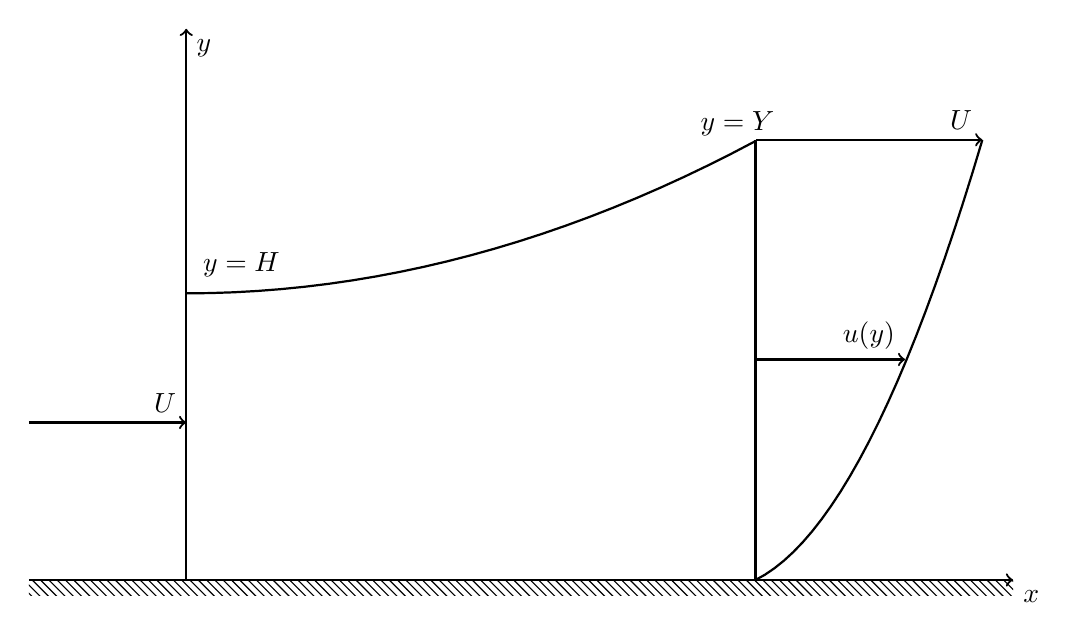
\begin{tikzpicture}
  \draw[thick, ->] (-4,-2) -- (8.5,-2) node[anchor=north west] {$x$};
  \draw[thick, ->] (-2,-2) -- (-2,5) node[anchor=north west] {$y$};

  \draw[thick] (5.23,-2) -- (5.23,3.59);

  \draw (-1.3,2) node {$y=H$};
  \draw (5.0,3.8) node {$y=Y$};



  \draw[thick, ->] (5.23,0.8) -- (7.13,0.8) node[anchor=south east] {$u(y)$};
  \draw[thick, ->] (-4,0) -- (-2,0) node[anchor=south east] {$U$};
  \draw[thick, ->] (5.23, 3.59) -- (8.11, 3.59) node[anchor=south east] {$U$};


  \fill[pattern=north west lines] (-4,-2.2) rectangle ++(12.5,0.2); 


  \begin{scope}[shift={(-2,1.64)}]
  \draw[thick, rotate=0, domain=0:7.23] plot ({\x},{0.037*\x*\x});
  \end{scope}


  \begin{scope}[shift={(5.23,-2)}]
    %\draw[thick, rotate=0, domain=0:2] plot ({\x},{sqrt(1 - \x*\x*0.5)});
  \draw[thick, rotate=0, domain=0:2.88] plot ({\x},{0.5*\x*\x + 0.5*\x});
  \end{scope}

\end{tikzpicture}

\end{center}
  \caption{Control volume for the analysis of flow past a flat plate} \label{fig:flat}
\end{figure}
\subsection*{Flat-Plate Integral Analysis}
This idea is based on considering flow of a viscous fluid at high \textit{Re} past a flat plate, as shown in Figure \ref{fig:flat}. The fluid will shear against the plate due to the no-slip condition and cause a frictional drag force $D$. The velocity profile $u(y)$ will at any given downstream position $x$ decline towards zero, as we move closer to the plate, as shown in the figure. Furthermore we are interested in finding the displacement thickness, which represent the amount of which streamlines outside the shear layer will deflect.
\subsection*{The Displacement Thickness}
We assume an incompressible flow, and by applying conservation of mass we can derive an expression for the boundary layer displacement thickness, $\delta^*$,
\begin{align}
  \delta^*(x) = \int_0^{Y \rightarrow \infty} \left( 1 - \frac{u}{U} \right)\, dy.
\end{align}
This relation holds true for any incompressible flow, wheter laminar or turbulent, constant or variable pressure and for constant or variable temperature.
\subsection*{The Momentum Thickness}
The displacement thickness can be derived by considering conservation of mass, while the momentum thickness can be reached by considering the momentum of the laminar boundary layer equations, and is defined as
\begin{align}
  \frac{D}{\rho U^2}  =\theta(x) = \int_0^{Y \rightarrow \infty} \frac{u}{U}\left( 1 - \frac{u}{U} \right)\, dy,
\end{align}
where $\rho$ is the density of the fluid and $D$ is the drag.
This relation holds true for any arbitrary incompressible boundary layer, but its relation to the drag varies, depending on if we have flat plate flow or not.

\subsection*{Drag and friction coefficients}
The two last parameters we need to define are the drag and friction coefficients. The general nondimensionalized version of these are as follows,\\\\
\text{Friction coefficient:}  
\[
  C_f = \frac{\tau_w(x)}{\frac{1}{2}\rho U^2}
\]
\text{Drag coefficient:} 
\[
  C_D = \frac{D}{\frac{1}{2} \rho U^2 L},
\]
where $L$ is the length of the plate, and $\tau_w$ is the wall shear stress. These equations can be adjusted if we consider a flat plate, which results in the following specialized form, 

\begin{align}
  C_{f,\text{plate}} &= 2 \frac{d \theta}{dx}\\[1.0em]
  C_{D, \text{plate}} &= 2 \frac{\theta(L)}{L} 
\end{align}
\subsection*{Assumed velocity profiles}
A guessed proile for computing numerical estimates is presented in the book \cite{frankwhite}. The example used throghout the text is a parabolic velocity profile, with corresponding values for $C_f$, $\theta$ and $\delta^*$, given by
\begin{align}
  u \approx U\left( \frac{2y}{\delta} - \frac{y^2}{\delta^2}\right),
\end{align}
where $U$ is the flow past a thin body and $\delta$ is the shear-layer thickness.
Using this profile the parameters which are computed result in a $\sim10\%$ error compared with the exact result from Blasius \cite{blasius}.\\\\
In this exercise we present an alternative velocity profile, first presented by Schlichting \cite{schli}. 
According to Schlichting, the flat-plate velocity profile
\[
  u \approx U\sin \left( \frac{\pi y}{2\delta} \right)
\]
gives a better accuracy for the parameters compared to (5). 
In addition to satisfying the standard boundary conditions, this profile also satiesfies $\partial^2 u / \partial y^2 = 0 $ at $y=0$.
Computing these parameters requires the relations from introductory boundary layer theory which are defined above. We start off by computing the displacement thickness,
\begin{align*}
  \delta^*(x) &= \int_0^{\delta} \left( 1 - \sin \left(\frac{\pi y}{2\delta} \right) \right)\, dy\\
  &= \delta \int_0^1 \left( 1 - \sin \left(\frac{\pi y^*}{2} \right) \right)\, dy, \qquad y^* = y / \delta\\
  &= \delta \left[ y^* + \frac{2}{\pi}\cos \left(\frac{\pi y^*}{2} \right) \right]^1_0\\
  &= \delta \left(1 - \frac{2}{\pi} \right)
\end{align*}
We can also express the momentum thickness, $\theta$, in terms of $\delta$,
\begin{align*}
  \theta(x) &= \int_0^{\delta} \sin \left( \frac{\pi y}{2 \delta} \right)\left( 1 - \sin \left( \frac{\pi y}{2 \delta} \right) \right) \, dy\\
  &= \delta\int_0^1 \left( \sin \left( \frac{\pi y^*}{2 } \right) - \sin^2 \left( \frac{\pi y^*}{2 } \right) \right)\, dy, \qquad y^* = y/\delta\\
  &= \delta \left[-\frac{2}{\pi}\cos \left( \frac{\pi y^*}{2}\right) - \frac{y^*}{2} + \frac{\sin(\pi y^*)}{2\pi}   \right]_0^1\\
  &= \delta \left(\frac{2}{\pi} - \frac{1}{2} \right)
\end{align*}
Furthermore we can compute the wall shear stress, $\tau_w$ as follows,
\begin{align*}
  \tau_w(x) &= \mu \frac{d u}{d y}\bigg|_{y=0}\\
  &=\mu \left( \frac{U\pi}{2 \delta} \cos \left(\frac{\pi y}{2\delta}\right) \right)\bigg|_{y=0}\\
  &= \frac{\mu U \pi}{2 \delta}
\end{align*}
We can now try to express $C_f$ to obtain a differential equation for $\delta$,
\begin{align*}
  C_f &= 2\frac{d\theta}{d x} = 2 \left(\frac{2}{\pi} - \frac{1}{2} \right) \frac{d \delta}{d x} \\ 
  &= \frac{\tau_w}{\frac{1}{2}\rho U^2} \\
  &= \frac{\frac{\mu U \pi}{2 \delta}}{\frac{1}{2}\rho U^2} \\
  &= \frac{\mu \pi}{\rho U} \frac{1}{\delta},
\end{align*}
which leads to the differential equation
\[
  \frac{\mu \pi}{\rho U} \left(\frac{2}{\pi} - \frac{1}{2} \right)^{-1} = \frac{d}{dx}(\delta^2)
\]
Integration from 0 to $x$ leads to the following relation, 
\[
  \delta^2 =  \frac{\mu \pi}{\rho U} \left(\frac{2}{\pi} - \frac{1}{2} \right)^{-1}x 
\]
or by taking the square root,
\[
  \delta(x)  = \sqrt{\frac{\mu \pi}{\rho U} \left(\frac{2}{\pi} - \frac{1}{2} \right)^{-1}} x^{\frac{1}{2}}
\]

\subsection*{Computation of the wall shear stress, $\tau_w(x)$}
With a final solution for $\delta$ we can now express $\tau_w$ as a function of $x$, 
\begin{align*}
  \tau_w(x) &= \frac{\mu U \pi}{2 \delta} \\
  &=   \frac{\mu U \pi}{2} \sqrt{\frac{\rho U}{\mu \pi} \left(\frac{2}{\pi} - \frac{1}{2} \right)} x^{-\frac{1}{2}}\\
  &=   \frac{1}{2} \sqrt{\rho \mu \pi U^3 \left(\frac{2}{\pi} - \frac{1}{2} \right)} x^{-\frac{1}{2}}
\end{align*}
\subsection*{Computation of the drag, $D$}
Finally we can compute the drag, $D$, given by
\[
  D = \int_0^L \tau_w(x)\, dx
\]
which by inserting the wall shear stress results in
\begin{align*}
  D &= \int_0^L  \frac{\mu U \pi}{2} \sqrt{\frac{\rho U}{\mu \pi} \left(\frac{2}{\pi} - \frac{1}{2} \right)} x^{-\frac{1}{2}}\, dx\\
  &=  \left[ \mu U \pi \sqrt{\frac{\rho U}{\mu \pi} \left(\frac{2}{\pi} - \frac{1}{2} \right)} x^{\frac{1}{2}}\right]^L_0\\
  &=  \mu U \pi \sqrt{\frac{\rho U}{\mu \pi} \left(\frac{2}{\pi} - \frac{1}{2} \right)} L^{\frac{1}{2}}\\
  &=  \sqrt{\rho \mu \pi L U^3 \left(\frac{2}{\pi} - \frac{1}{2} \right)} 
\end{align*}

\subsection*{Log-log plot of Drag coefficient vs. Reynolds number}
By running the following Python-script, we get a visualization of the drag coefficient, $C_f$, plotted against the Reynolds number, $Re$, with values of $Re$ ranging from 1000 to 10000. 
\lstinputlisting{loglog.py}
Running the script produces the following log-log plot:
\begin{center}
\includegraphics{loglog}
\end{center}

\subsection*{Comparisson with Blasius' exact solution}
To finally verify that this solution is an improvement, we will compare the following values with the exact values given by Blasius,
\[
  \frac{\theta}{x}\sqrt{Re_x},\quad 
  \frac{\delta^*}{x}\sqrt{Re_x}, \quad
  \frac{\delta}{x}\sqrt{Re_x}, \quad
  C_f\sqrt{Re_x}, \quad
  C_D\sqrt{Re_L},
\]
where $Re_x = \rho U x / \mu$.
With our exact solution of $\delta$, we can express $\theta$ and $\delta^*$ since these quantities are depenent of $\delta$. This leads to the following values of the parameters above,
\[
  \frac{\theta}{x}\sqrt{Re_x} = \frac{\delta}{x} \left( \frac{2}{\pi} - \frac{1}{2} \right)\sqrt{Re_x} =
  \left( \frac{2}{\pi} - \frac{1}{2} \right)\sqrt{\pi \left( \frac{2}{\pi} - \frac{1}{2} \right)^{-1}}  = 0.655
\]

which is only an error of 1.35\% compared to the exact result of 0.664.
Similarly we can find $\delta^*/x \sqrt{Re_x}$, 

\[
  \frac{\delta^*}{x}\sqrt{Re_x} = \frac{\delta}{x} \left( 1 - \frac{2}{\pi}  \right)\sqrt{Re_x} =
  \left( 1 - \frac{2}{\pi}  \right)\sqrt{\pi \left( \frac{2}{\pi} - \frac{1}{2} \right)^{-1}}  = 1.742
\]

which is only an error of 1.23\% compared to the exact result of 1.721.
Furthermore, 

\[
  \frac{\delta}{x}\sqrt{Re_x} 
= \sqrt{\pi \left( \frac{2}{\pi} - \frac{1}{2} \right)^{-1}}  = 4.795
\]
which is an error of 4.09\% compared to the exact result of 5.
We can also fully express $C_f$ or $C_f \sqrt{Re_x}$, 
\[
  C_f = 2\frac{d\theta}{d x} = 2 \left(\frac{2}{\pi} - \frac{1}{2} \right) \frac{d \delta}{d x} =    2 \left(\frac{2}{\pi} - \frac{1}{2} \right) \frac{1}{2} \sqrt{\frac{\mu \pi}{\rho U} \left(\frac{2}{\pi} - \frac{1}{2} \right)^{-1}} x^{-\frac{1}{2}} \approx \frac{0.655}{\sqrt{Re_x}}
\]
or equivalently
\[
  C_f \sqrt{Re_x} = 0.655,
\]
which is only an error of 1.35\% compared to the exact result of 0.664.
Finally we express the drag coefficient ratio,
\[
  C_D\sqrt{Re_L} = \frac{2}{L}\theta(L)\sqrt{Re_L} = \frac{2\sqrt{Re_L}}{L} \left( \frac{2}{\pi} - \frac{1}{2} \right) \delta(L) = 2 \left( \frac{2}{\pi} - \frac{1}{2} \right) \sqrt{\pi \left( \frac{2}{\pi} - \frac{1}{2} \right)^{-1}} = 1.310
\]
which is only an error of 1.33\% compared to the exact result of 1.328.
These calculations lead to the following table, which shows a comparisson between our guessed profile and the exact solution by Blasius.


\begin{center}
\begin{tabular}{l*{4}{c}}
  \toprule
  \thead{\textbf{ Parameter} }& \thead{\textbf{ u(y) proposed} \\ \textbf{by Schlichting}} & \thead{\textbf{Exact from} \\ \textbf{ Blasius}} & \textbf{Error, \%}\\
  \midrule
  $\frac{\theta}{x}\sqrt{Re_x}$ &  0.655 & 0.664 & +1.35\\[0.7em]
  $\frac{\delta^*}{x}\sqrt{Re_x}$ & 1.742 & 1.721 & +1.23\\[0.7em]
  $\frac{\delta}{x}\sqrt{Re_x}$  & 4.795 & 5.0 & +4.09\\[0.7em]
  $C_f\sqrt{Re_x}$ &	0.655 & 0.664 & +1.35\\[0.7em]
  $C_D\sqrt{Re_L}$ &	1.310 & 1.328 & +1.33\\
  \bottomrule
\end{tabular}
\end{center}

\begin{thebibliography}{9}

 \bibitem{frankwhite}
    White, F. M., Viscous Fluid Flow, 3rd Edition, McGraw-Hill, New York, 2006.
    
  \bibitem{blasius}
    Blaius, H., Grenzschichten in Flüsikeiten mit kleiner Reibung, Z. Angew. Math. Phys., vol.56, 1908.

  \bibitem{schli}
    Schlichting, H., Boundary Layer Theory, 7th. Edition, McGraw-Hill, New York, 1979
\end{thebibliography}





\end{document}
